\documentclass[10pt,twocolumn,a4paper]{article}
% Kompilacja: pdfLaTeX + BibTeX (np. Overleaf).
\usepackage[T1]{fontenc}
\usepackage[utf8]{inputenc}
\usepackage{polski,lmodern}
\usepackage[margin=18mm,columnsep=7mm]{geometry}
\usepackage{microtype,graphicx}
\usepackage{booktabs,tabularx,array}
\usepackage{amsmath,amssymb}
\usepackage{enumitem,placeins,xcolor,xurl,float,needspace,etoolbox}
\usepackage[font=footnotesize,labelfont=bf,skip=4pt]{caption}
\usepackage[hidelinks,breaklinks=true]{hyperref}
\hypersetup{pdftitle={Predykcja rzeczywistego zużycia paliwa samochodów osobowych}}
\setlist[itemize]{leftmargin=*,itemsep=1pt,topsep=3pt}
\setlist[description]{leftmargin=0pt,labelsep=4pt,itemsep=3pt}
\setlength{\emergencystretch}{1em}
\raggedbottom
\pretocmd{\section}{\Needspace{6\baselineskip}}{}{}
\pretocmd{\subsection}{\Needspace{5\baselineskip}}{}{}
\newcolumntype{Y}{>{\raggedright\arraybackslash}X}
\renewcommand{\abstractname}{Streszczenie}
\renewcommand{\refname}{Bibliografia}
\graphicspath{{figures/}}

\newcommand{\TematProjektu}{Predykcja rzeczywistego zużycia paliwa samochodów osobowych na podstawie danych OBFCM}
\newcommand{\TypZadania}{Regresja}
\newcommand{\lkm}{\,l/100\,km}

\title{\TematProjektu\\[2mm]
\large Zaawansowane metody uczenia maszynowego}
\author{Imię i nazwisko autora 1\\\small Numer albumu
\and Imię i nazwisko autora 2\\\small Numer albumu}
\date{\quad \today}
\begin{document}
\maketitle

\begin{abstract}
Katalogowe zużycie paliwa wyznaczane w procedurze WLTP (ang.\ \emph{Worldwide
Harmonised Light Vehicles Test Procedure}) systematycznie zaniża spalanie
w codziennej eksploatacji. Celem projektu jest model regresyjny, który na
podstawie parametrów technicznych i homologacyjnych pojazdu przewiduje jego
rzeczywiste średnie zużycie paliwa. Wykorzystujemy dane z pokładowych urządzeń
monitorujących zużycie paliwa OBFCM (ang.\ \emph{On-Board Fuel Consumption
Monitoring}) dla 7,7 mln samochodów spalinowych i hybrydowych zarejestrowanych
w Unii Europejskiej w latach 2021--2024. Dane podzielono grupowo według modelu
samochodu, aby ocena odpowiadała predykcji dla modelu nieobecnego w danych
uczących. Miarą główną jest średni błąd bezwzględny MAE (ang.\ \emph{Mean
Absolute Error}). Model bazowy \texttt{HistGradientBoosting} bez strojenia
osiąga na zbiorze testowym MAE 0,61\lkm, wobec 0,69\lkm{} dla katalogowego
zużycia paliwa skorygowanego regresją liniową i 1,16\lkm{} dla samej wartości
katalogowej. Przewaga modelu utrzymuje się w każdym z 5 losowych podziałów.
Ograniczeniem są różnice w stylu jazdy: egzemplarze tego samego auta spalają
różnie zależnie od kierowcy, a model widzi tylko cechy auta. Nawet idealna
znajomość typowego zużycia paliwa każdej wersji auta dawałaby błąd ok.\
0,52\lkm{} -- to dolna granica, której żaden model oparty na cechach
technicznych nie przekroczy.
\end{abstract}

\section{Problem, motywacja i cel}
\subsection{Pytanie predykcyjne}
Oficjalne zużycie paliwa wyznaczane jest w laboratorium w procedurze WLTP
(ang.\ \emph{Worldwide Harmonised Light Vehicles Test Procedure} -- światowa
zharmonizowana procedura badania pojazdów lekkich): w stałej temperaturze,
według ustalonego profilu prędkości i z wyłączonymi odbiornikami energii.
Wynik tego testu producent podaje jako oficjalne, \emph{katalogowe zużycie
paliwa}. W ruchu drogowym zużycie paliwa jest wyższe. Różnicę między
rzeczywistym a katalogowym zużyciem paliwa nazywamy dalej \emph{luką}.
Według raportów Komisji Europejskiej i ICCT (ang.\ \emph{International
Council on Clean Transportation}) luka dla aut spalinowych i hybrydowych
wynosi ok.\ 18--21\% \cite{ec2024report,diaz2026obfcm}. Od 2021 r. nowe
pojazdy w Unii Europejskiej (UE) rejestrują skumulowane zużycie paliwa
i przebieg za pomocą urządzeń OBFCM (ang.\ \emph{On-Board Fuel Consumption
Monitoring} -- pokładowe monitorowanie zużycia paliwa), a dane te są
publikowane \cite{reg2019_631,eea2024obfcm}. Pozwala to nauczyć model, który
przewiduje rzeczywiste zużycie paliwa bezpośrednio z parametrów pojazdu.

\noindent\textbf{Typ zadania:} \TypZadania.

\noindent\textbf{Kontrakt predykcji:}
\begin{itemize}
\item \emph{jednostka obserwacji:} pojedynczy samochód osobowy (spalinowy lub
hybryda bez ładowania z sieci) zarejestrowany w UE,
\item \emph{moment predykcji:} przed rozpoczęciem eksploatacji -- znane są
wyłącznie dane homologacyjne, kraj i rok rejestracji,
\item \emph{cechy:} masa, masa testowa, pojemność, moc, emisja dwutlenku węgla
(CO$_2$) i zużycie paliwa z testu WLTP, rodzaj paliwa, typ napędu, kategoria,
marka, kraj, wiek pojazdu,
\item \emph{cel:} średnie rzeczywiste zużycie paliwa w całym okresie
eksploatacji [l/100\,km],
\item \emph{zastosowanie:} realistyczna informacja dla kupujących i flot oraz
szacowanie rzeczywistej emisji dla nowych modeli, zanim pojawią się dla nich
dane OBFCM.
\end{itemize}

\subsection{Kryterium użyteczności}
Aby ocenić, czy model wnosi coś nowego, porównujemy go z \emph{modelami
bazowymi} (ang.\ \emph{baseline}). Są to możliwie najprostsze sposoby
przewidywania, dostępne bez uczenia maszynowego. Model ma sens, jeśli
przewiduje wyraźnie lepiej niż one: (1) stała wartość (mediana), (2) katalogowe
zużycie paliwa oraz (3) katalogowe zużycie paliwa skorygowane prostą regresją
liniową osobno dla czterech segmentów: benzyna/diesel $\times$ napęd
spalinowy/hybrydowy. Trzeci punkt odniesienia odpowiada korekcie luki
stosowanej w analizach regulacyjnych („rzeczywiste = katalogowe + $x$\%”),
więc to z nim porównujemy model w pierwszej kolejności.

\section{Dane i analiza wstępna}
\subsection{Źródło i znaczenie kolumn}
Zbiór \texttt{2024\_Cars\_Raw.csv} opublikowała Europejska Agencja Środowiska
EEA (ang.\ \emph{European Environment Agency}) \cite{eea2024obfcm}.
Monitorowanie rzeczywistej emisji samochodów osobowych i dostawczych opiera się
na art.~12 rozporządzenia (UE) 2019/631 \cite{reg2019_631}. Jego celem jest
sprawdzanie, czy emisje CO$_2$ wyznaczone w laboratorium pozostają
reprezentatywne dla emisji pojazdów w ruchu. Dane zostały pobrane
w październiku 2026 r. z serwisu \url{https://sdi.eea.europa.eu}, a EEA
udostępnia je do ponownego wykorzystania z podaniem źródła. Plik zawiera
10\,810\,654 rekordy i 32 kolumny: odczyty liczników OBFCM przekazane przez
producentów lub państwa członkowskie, połączone z danymi homologacyjnymi
pojazdu.

Populację zawężono do rekordów zaakceptowanych przez EEA
(\texttt{Used in calculation} = 1) i do napędów M (spalinowy) oraz H (hybryda
klasyczna). Pojazdy elektryczne nie zużywają paliwa, a hybrydy plug-in łączą
paliwo z energią z sieci, co zmienia znaczenie celu. Po zawężeniu pozostaje
7\,745\,790 rekordów. Kolumny paliwa i przebiegu zostały usunięte z cech, bo
wyznaczają cel (wyciek informacji). Pominięto też identyfikatory i metadane
administracyjne. Kluczowe kolumny przedstawia tab.~\ref{tab:dane}.

\begin{table}[H]
\centering
\caption{Skrócony słownik danych: znaczenie, jednostka i dostępność.}
\label{tab:dane}
\footnotesize
\renewcommand{\arraystretch}{1.45}
\begin{tabularx}{\columnwidth}{@{}lYY@{}}
\toprule
Kolumna & Znaczenie / jednostka & Rola / dostępność\\
\midrule
\texttt{M (kg)}, \texttt{Mt} & masa własna, masa testowa WLTP [kg] & cecha, homologacja\\
\texttt{Ec (cm3)} & pojemność silnika [cm$^3$] & cecha, homologacja\\
\texttt{Ep (KW)} & moc maksymalna [kW] & cecha, homologacja\\
\texttt{Ewltp (g/km)} & emisja CO$_2$ w teście WLTP [g/km] & cecha, homologacja\\
\texttt{Fuel consumption} & katalogowe zużycie paliwa [l/100\,km] & cecha, homologacja\\
\texttt{Ft}, \texttt{Fm} & rodzaj paliwa; napęd M -- spalinowy, H -- hybryda & cechy nominalne\\
\texttt{Cr} & kategoria: M1 -- osobowy, M1G -- terenowy & cecha nominalna\\
\texttt{Mk}, \texttt{Country} & marka, kraj rejestracji & cechy nominalne\\
\texttt{Year} & rok rejestracji 2021--2024 & cecha (wiek pojazdu)\\
\texttt{Cn} & nazwa handlowa modelu & tylko do podziału\\
\texttt{Total fuel / distance} & paliwo [l] i przebieg [km] w okresie eksploatacji & tylko do wyznaczenia celu\\
\texttt{real\_fuel\_consumption} & $100\cdot$paliwo/przebieg [l/100\,km] & zmienna zależna\\
\bottomrule
\end{tabularx}
\end{table}

\subsection{Jakość i struktura danych}
W wybranych kolumnach nie ma duplikatów ani pustych celów. Wykryto natomiast
trzy rodzaje błędów:
\begin{itemize}
\item \emph{niespójne kodowanie} -- ten sam rodzaj paliwa zapisano jako
\texttt{petrol}/\texttt{PETROL} (1\,953\,445 rekordów zapisanych wielkimi
literami); ujednolicono wielkość liter,
\item \emph{sprzeczność logiczna masy} -- masa testowa mniejsza od masy własnej
lub większa o ponad 1000\,kg (9\,465 wartości),
\item \emph{sprzeczność wartości z testu WLTP} -- emisja CO$_2$ i zużycie
paliwa pochodzą z tego samego testu, a spalenie litra danego paliwa zawsze
daje praktycznie tę samą ilość CO$_2$. Iloraz emisji i zużycia paliwa
powinien więc być stały dla benzyny i osobno dla oleju napędowego
(rys.~\ref{fig:spojnosc}). Odchylenie o ponad 15\% od typowej wartości
(235\,225 wartości, 3,0\%) uznano za błąd wpisu.
\end{itemize}
Błędne wartości zamieniono na braki (nie usuwano wierszy, bo cel i pozostałe
cechy są poprawne) i uzupełniono imputacją dopasowaną na zbiorze treningowym
(rozdz.~\ref{sec:imp}).

Wartości poza wąsami wykresu pudełkowego, czyli dalej niż 1,5 rozstępu
międzykwartylowego IQR (ang.\ \emph{interquartile range}) od kwartyli,
występują w 10,8\% wierszy co najmniej w jednej kolumnie. Są to jednak realne,
duże i mocne pojazdy, a nie błędy, więc nie stosujemy reguły IQR. Usuwamy tylko
wartości fizycznie niemożliwe, z granicami ustalonymi \emph{a priori}: zużycie
paliwa 0,5--35\lkm, masa 500--4500\,kg, pojemność 500--8000\,cm$^3$, moc
20--1000\,kW. Odrzucono 21\,060 rekordów (0,27\%), po czym zostaje
7\,724\,730 wierszy.

Braków jest niewiele, poza katalogowym zużyciem paliwa: w zbiorze treningowym
brakuje 9,4\% wartości \texttt{Fuel consumption} (łącznie z oznaczonymi jako
błędne), 0,54\% \texttt{Mt} i 0,09\% \texttt{Ep}. Braki katalogowego zużycia
paliwa zależą od rocznika (27,6\% w 2021 r., poniżej 5\% później)
i producenta. Są więc typu MAR (ang.\ \emph{Missing At Random} -- brak zależny
od obserwowanych zmiennych), a nie MCAR (ang.\ \emph{Missing Completely At
Random} -- brak całkowicie losowy) \cite{little2019missing}.

Rozkład celu (rys.~\ref{fig:cel}) jest jednomodalny i prawostronnie skośny:
mediana 6,78\lkm, średnia 7,15\lkm, skośność 2,64. Cechy techniczne również
mają prawe ogony, a pojemność i moc są wielomodalne (standardowe wersje
silników). Logarytm zmniejsza skośność, np. pojemności z 1,64 do 0,30 i mocy
z 2,65 do 0,78.

\begin{figure}[H]
\centering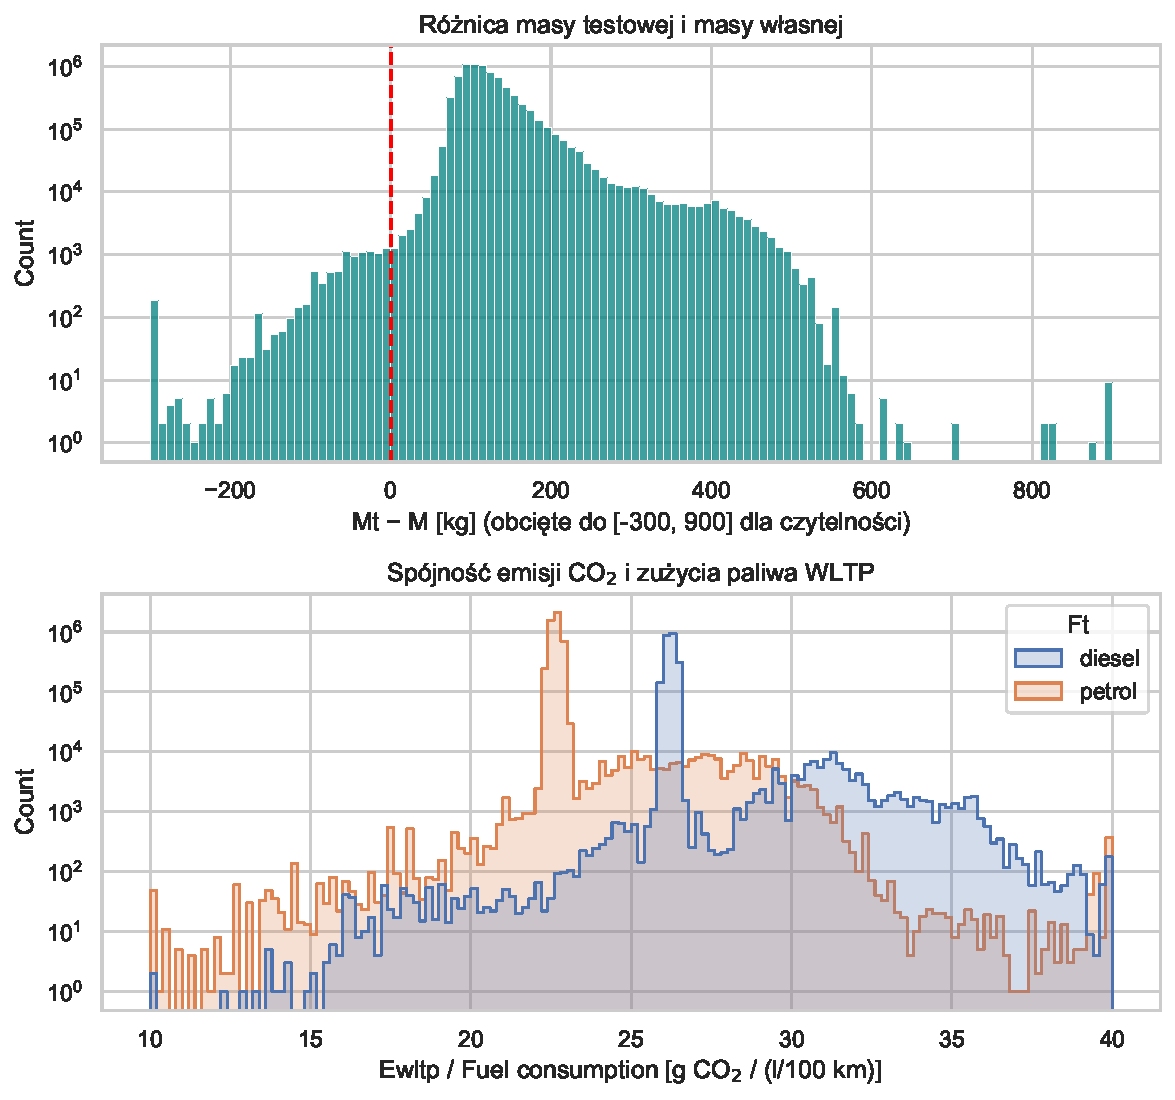
\includegraphics[width=\columnwidth]{consistency_checks}
\caption{Kontrole spójności. Góra: różnica masy testowej i własnej.
Dół: iloraz emisji CO$_2$ i zużycia paliwa z testu WLTP -- piki przy 22,7
(benzyna) i 26,2 (diesel) wynikają ze składu paliwa, wartości poza nimi są
błędnymi wpisami.}
\label{fig:spojnosc}
\end{figure}

\begin{figure}[H]
\centering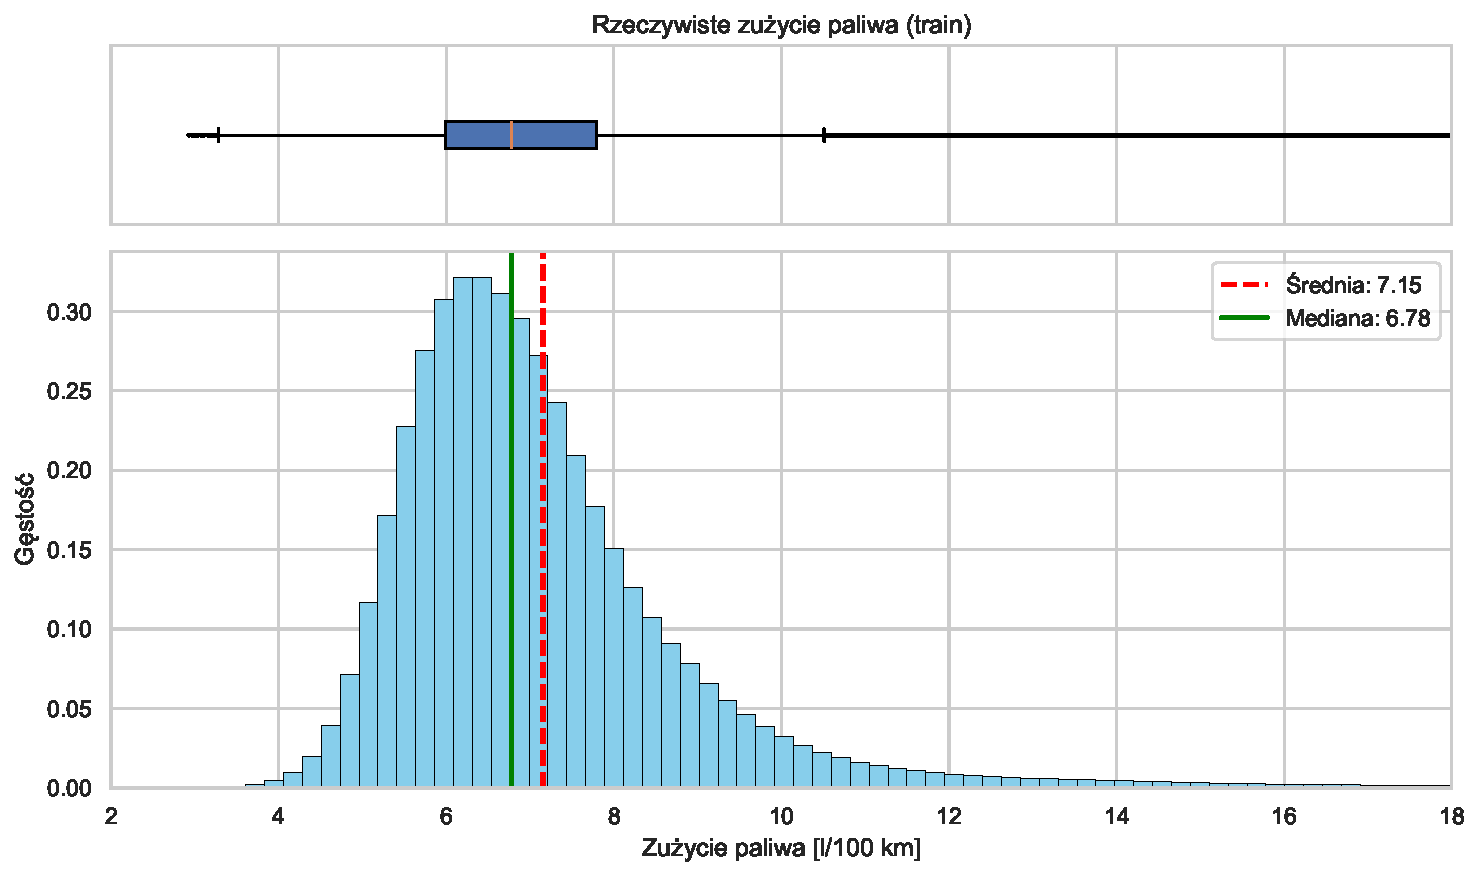
\includegraphics[width=\columnwidth]{target_distribution}
\caption{Rozkład rzeczywistego zużycia paliwa (zbiór treningowy).}
\label{fig:cel}
\end{figure}

\subsection{Najważniejsze obserwacje z EDA}
Eksploracyjną analizę danych EDA (ang.\ \emph{Exploratory Data Analysis})
wykonano wyłącznie na zbiorze treningowym.
\begin{itemize}
\item 85,3\% pojazdów spala więcej paliwa, niż deklaruje producent. Średnia
luka wynosi +1,17\lkm{} (mediana +1,02\lkm).
\item Z rzeczywistym zużyciem paliwa najsilniej korelują katalogowe zużycie
paliwa i emisja CO$_2$ z testu WLTP (współczynnik Pearsona 0,87 i 0,81),
a dalej moc (0,73), pojemność (0,51) i masa (0,47). Katalogowe zużycie paliwa
i emisja CO$_2$ są niemal redundantne, a wiek pojazdu jest praktycznie
nieskorelowany z celem ($-0,03$).
\item Rys.~\ref{fig:multi} pokazuje, że luka nie jest stałym przesunięciem:
zależy od segmentu paliwo$\times$napęd i rośnie z masą i mocą. Dlatego model
nieliniowy może poprawić prostą korektę katalogowego zużycia paliwa.
\item Mediana zużycia paliwa różni się między krajami rejestracji
(6,0--8,8\lkm). To obserwacja, a nie zależność przyczynowa: kraje różnią się
strukturą tras, klimatem i sprzedawanymi modelami.
\end{itemize}
Wykresy pudełkowe, histogramy, wykres par cech, macierze korelacji i rozkłady
cech kategorycznych znajdują się w notatniku.

\begin{figure}[H]
\centering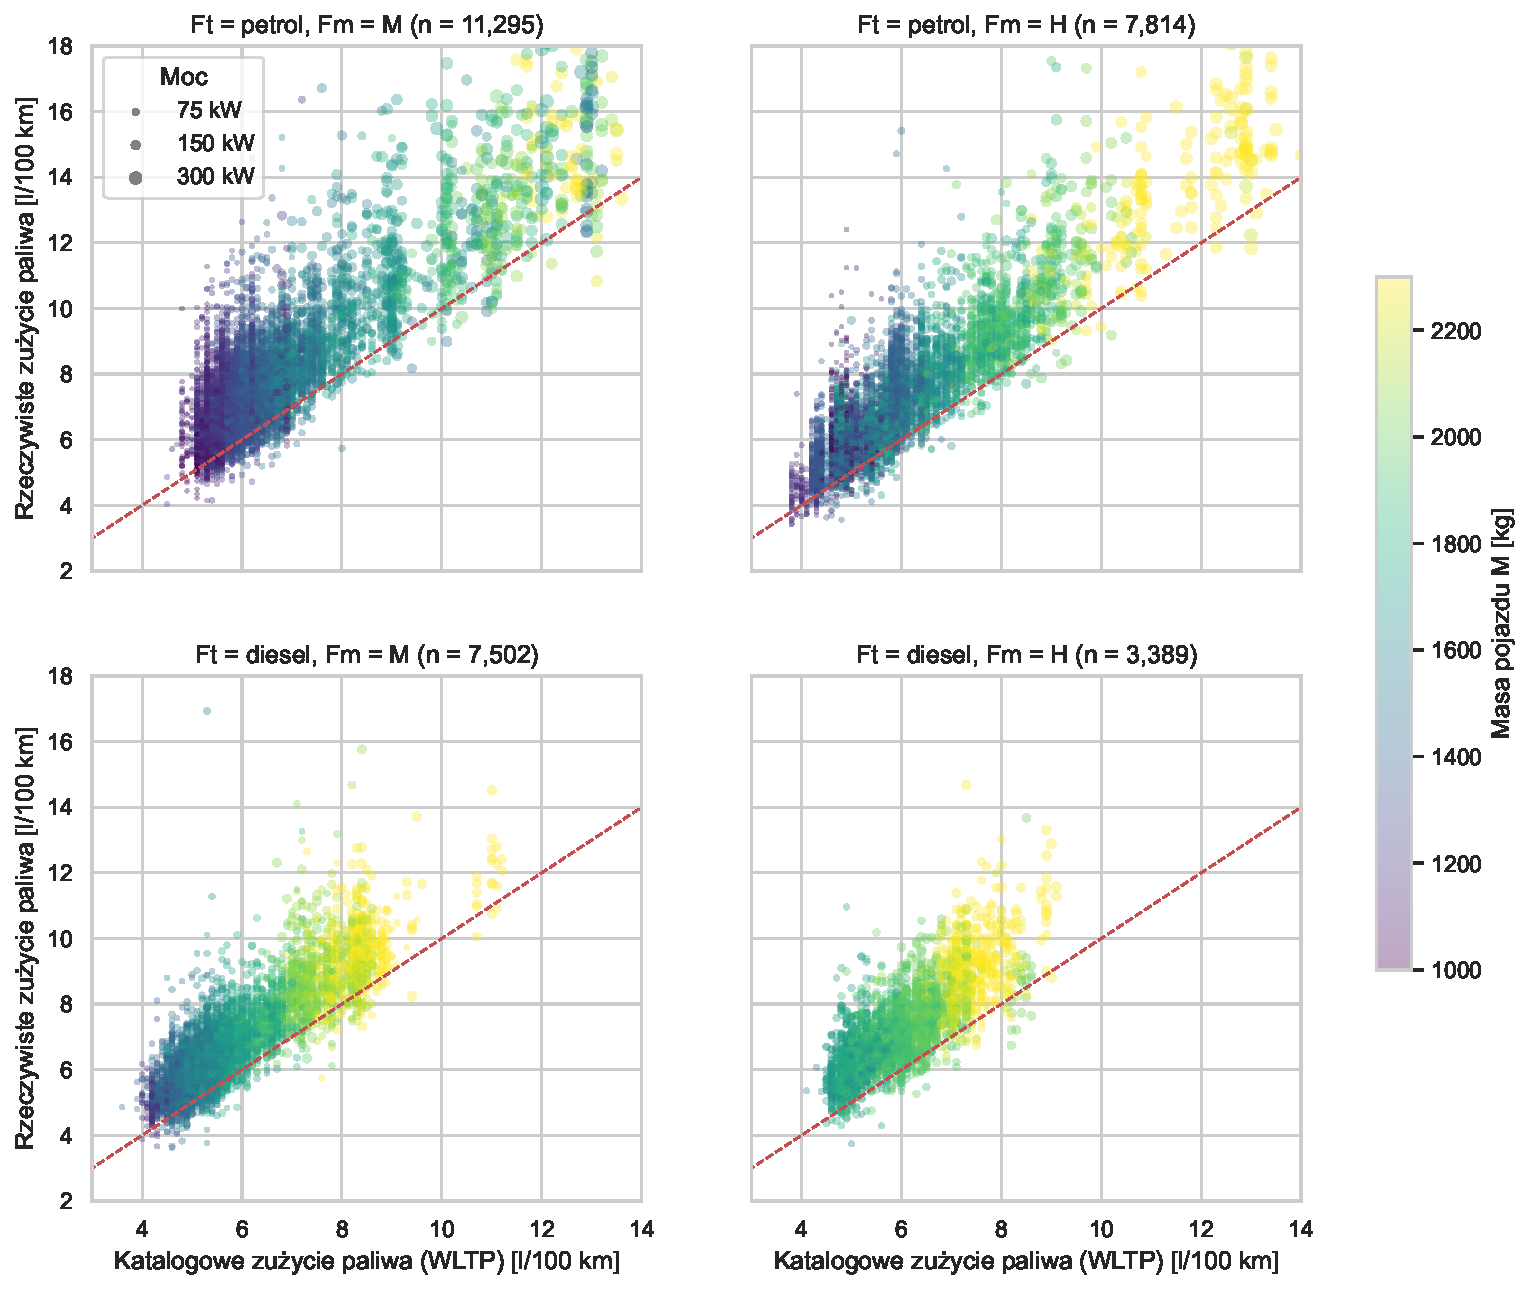
\includegraphics[width=\columnwidth]{multivariate}
\caption{Katalogowe a rzeczywiste zużycie paliwa w 4 segmentach
(paliwo$\times$napęd); kolor -- masa, rozmiar -- moc; linia przerywana: $y=x$.
Próba 30\,tys. pojazdów ze zbioru treningowego.}
\label{fig:multi}
\end{figure}

\section{Przegląd literatury}
Rozbieżność między laboratoryjnym a drogowym zużyciem paliwa w Europie opisuje
przegląd Fontarasa i in. \cite{fontaras2017fuel}. Jej źródła to
m.in.\ procedura testowa, temperatura, odbiorniki energii i styl jazdy.
ICCT na danych z serwisów użytkowników (ok.\ 1,3 mln aut) pokazało wzrost
luki z 9\% w 2001 r.\ do 39\% w 2017 r.\ dla wcześniejszej procedury NEDC
(ang.\ \emph{New European Driving Cycle} -- nowy europejski cykl jezdny)
\cite{tietge2019lab}. Pavlovic i in. \cite{pavlovic2020gap} przez rok
monitorowali jeden pojazd prowadzony przez 20 kierowców (ok.\ 14\,tys.\,km).
Luka wyniosła 29\%, a regresja na cechach przejazdu (prędkość, nachylenie,
długość trasy, kierowca) wyjaśniała ok.\ 90\% jej zmienności. Pokazuje to,
że duża część zmienności zużycia paliwa wynika z warunków użytkowania, a nie
z cech pojazdu.

Dane OBFCM są analizowane od 2021 r. Komisja Europejska \cite{ec2024report}
raportuje lukę ok.\ 1,2--1,3\lkm{} dla benzyny. Díaz i in.
\cite{diaz2026obfcm} na ok.\ 8 mln aut z lat 2021--2023 podają lukę
18--19\% dla napędów spalinowych i hybrydowych. Suarez Corujo i in.
\cite{suarez2025onboard} budują wielowymiarowe modele regresji dla 7,7 mln
aut i wskazują masę i moc jako główne źródła zmienności emisji pojazdów
spalinowych i hybrydowych. Wyniki te zgadzają się z naszą EDA, ale dotyczą
średnich flotowych, a nie predykcji dla pojedynczego modelu.

Uczenie maszynowe do predykcji rzeczywistego zużycia paliwa stosowano na
danych zgłaszanych przez właścicieli aut w Chinach. Zeng i in.
\cite{zeng2021estimation} uzyskali najlepszy wynik modelem LightGBM (ang.\
\emph{Light Gradient Boosting Machine} -- gradientowe wzmacnianie drzew
decyzyjnych) \cite{ke2017lightgbm}: MAE 0,911\lkm, $R^2$ 0,642. Najważniejsze
cechy to referencyjne zużycie paliwa, moc i marka. Yang i in.
\cite{yang2022predicting}, dodając cechy stylu jazdy i otoczenia, uzyskali
lasem losowym MAE 0,630\lkm. Wyniki te nie są bezpośrednio porównywalne
z naszymi (inna populacja, cykl referencyjny i podział danych), ale wskazują
rząd wielkości błędu i przewagę modeli drzewiastych.

W części metodycznej opieramy się na pracach o imputacji MICE
\cite{vanbuuren2011mice} i KNN \cite{troyanskaya2001knn}, o podziale danych
o strukturze hierarchicznej \cite{roberts2017cv} oraz o wycieku informacji
\cite{kaufman2012leakage}. Implementacja wykorzystuje bibliotekę
scikit-learn \cite{pedregosa2011sklearn}.

\section{Protokół eksperymentu}
\subsection{Podział i granica dopasowania}
Wiersz to pojedynczy egzemplarz pojazdu, ale cechy techniczne są wspólne dla
wszystkich egzemplarzy wariantu: na 7,7 mln wierszy przypada ok.\ 149 tys.
unikalnych kombinacji cech. Przy podziale losowym ten sam wariant trafiłby do
treningu i testu, a model mógłby zapamiętać jego średnie zużycie paliwa. Wynik
byłby wtedy zawyżony. Docelowe użycie to predykcja dla \emph{nowego} modelu
samochodu, dlatego dzielimy \textbf{grupowo po modelu} (marka + nazwa
handlowa, 5\,898 grup): wszystkie wersje i rejestracje danego modelu trafiają
do jednej części. Grupy są losowo permutowane (ziarno 42) i przydzielane tak,
aby proporcje wierszy były bliskie 70/15/15. Uzyskano 5\,167\,110 /
1\,444\,907 / 1\,112\,713 wierszy (66,9 / 18,7 / 14,4\%, rys.~\ref{fig:split}).
Odchylenie wynika z tego, że pojedynczy model może obejmować ponad 100 tys.
egzemplarzy, a grup nie dzielimy. Z tego samego powodu różni się skład
segmentów: w walidacji jest tylko ok.\ 2\% hybryd z silnikiem diesla (w treningu
ok.\ 11\%) i więcej aut benzynowych, przez co rozkład zużycia paliwa jest tam
węższy. Dlatego wyniki sprawdzono także dla kilku losowych podziałów
(rozdz.~\ref{sec:stab}). Podział czasowy nie jest adekwatny, bo
wszystkie odczyty pochodzą z jednego okresu raportowego (2024), a rok
rejestracji opisuje wiek pojazdu.

\paragraph{Kontrola przenikania informacji.} Sprawdzono, że żaden model
samochodu ani żaden pojedynczy pojazd nie występuje w więcej niż jednej części
zbioru. Dodatkowo sprawdzono, ile pojazdów z walidacji i testu ma dokładnie
takie same parametry techniczne (marka, paliwo, napęd, kategoria, masa,
pojemność, moc, emisja CO$_2$) jak jakiś pojazd treningowy. Dotyczy to
33,6\% wierszy walidacji i 52,4\% wierszy testu. Wynika to z tego, że
producenci montują ten sam silnik w kilku modelach tej samej marki. Nie
traktujemy tego jako wycieku: nowy model samochodu zwykle dostaje silnik znany
już z innych modeli, więc taka sytuacja odpowiada docelowemu zastosowaniu.
Przypisanie wierszy do części utrwalono w pliku
\texttt{splits/split\_seed42.csv.gz}.

\paragraph{Rola części zbioru.}
\begin{itemize}
\item \textbf{Train:} dopasowanie preprocessingu i modeli, EDA, wybór imputacji.
\item \textbf{Validation:} porównanie wariantów i modeli bazowych.
\item \textbf{Test:} jednorazowa ocena zamrożonej procedury.
\end{itemize}

Reguły czyszczenia z rozdz.~2.2 są deterministyczne i nie korzystają
z rozkładu danych, dlatego zastosowano je przed podziałem. Wszystkie uczone
transformacje (imputacja, skalowanie, kodowanie) są częścią potoku
\texttt{Pipeline} i dopasowują się wyłącznie do części treningowej.

\begin{figure}[H]
\centering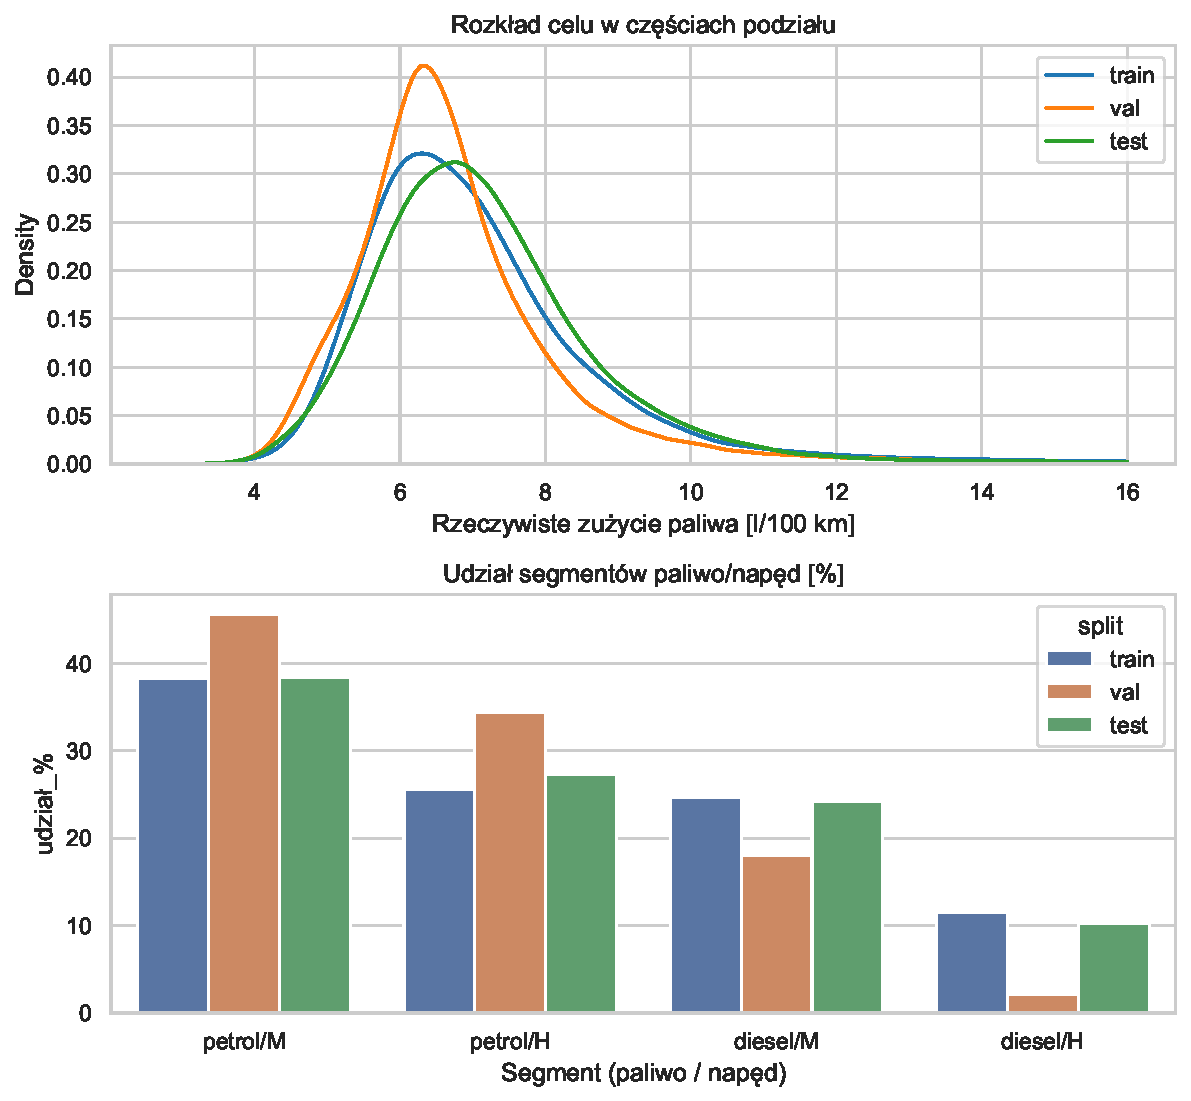
\includegraphics[width=\columnwidth]{split_check}
\caption{Rozkład rzeczywistego zużycia paliwa (góra) i udział segmentów
paliwo/napęd (dół) w częściach podziału grupowego.}
\label{fig:split}
\end{figure}

\subsection{Metryka główna i miary pomocnicze}
\noindent\textbf{Miara główna:} MAE (ang.\ \emph{Mean Absolute Error} --
średni błąd bezwzględny) [l/100\,km], im mniej, tym lepiej. Jest w jednostce
celu („średnio mylimy się o $x$ litrów na 100\,km”) i jest odporna na długi
prawy ogon tworzony przez nietypowych kierowców, których cechy pojazdu nie
opisują.

\noindent\textbf{Miary pomocnicze:}
\begin{itemize}
\item RMSE (ang.\ \emph{Root Mean Squared Error} -- pierwiastek błędu
średniokwadratowego) [l/100\,km] -- silniej karze duże błędy,
\item mediana błędu bezwzględnego [l/100\,km] -- błąd typowego pojazdu,
\item MAPE (ang.\ \emph{Mean Absolute Percentage Error} -- średni bezwzględny
błąd procentowy) [\%] -- porównanie aut małych i dużych,
\item $R^2$ (współczynnik determinacji) -- część wyjaśnionej wariancji, może
być ujemny,
\item średni błąd (bias) [l/100\,km] -- czy model, podobnie jak katalogowe
zużycie paliwa, systematycznie zaniża spalanie.
\end{itemize}

\section{Preprocessing i baseline}\label{sec:prep}
\subsection{Potok przetwarzania}
Potok preprocessingu stosuje kolejno, osobno dla każdego typu zmiennych:
\begin{enumerate}[leftmargin=*,itemsep=1pt]
\item \emph{liczbowe} (masa, masa testowa, pojemność, moc, emisja CO$_2$,
katalogowe zużycie paliwa): logarytm, imputacja MICE ze wskaźnikami braku,
standaryzacja; wiek pojazdu ($2024-$\texttt{Year}) bez logarytmu,
\item \emph{nominalne binarne} (\texttt{Ft}, \texttt{Fm}, \texttt{Cr}):
dominanta, kodowanie zero-jedynkowe (one-hot) z pominięciem jednej kategorii,
\item \emph{nominalne wielopoziomowe} (\texttt{Country}, \texttt{Mk}):
kodowanie one-hot; kategorie z udziałem $<0,1\%$ (np. 109 ze 146 marek)
łączone są w jedną, a kategorie niewidziane traktowane jak rzadkie.
\end{enumerate}

\subsection{Imputacja braków}\label{sec:imp}
Porównano 3 metody podstawowe (średnia, mediana, dominanta) i 2 zaawansowane:
KNN (ang.\ \emph{k-Nearest Neighbors} -- $k=5$ najbliższych sąsiadów) oraz
MICE (ang.\ \emph{Multiple Imputation by Chained Equations} -- imputacja
łańcuchem równań regresji). W MICE każda kolumna z brakami jest przewidywana
regresją z pozostałych kolumn, a cykl powtarza się, aż wartości się
ustabilizują. Ocenę przeprowadzono na 40\,tys. kompletnych wierszy
treningowych, w których sztucznie usunięto (całkowicie losowo, ziarno 42) po
20\% wartości \texttt{Fuel consumption}, \texttt{Ep} i \texttt{Mt}. Dane
oryginalne pozostały bez zmian.

Najdokładniej usunięte wartości odtwarza KNN (MAE katalogowego zużycia paliwa
0,06\lkm), dalej MICE (0,26\lkm). Metody proste mylą się o ok.\ 0,9\lkm,
wstawiają jedną wartość i zaniżają wariancję o ok.\ 10\% (sztuczne piki na
rys.~\ref{fig:imp}). Wpływ na model jest jednak niewielki: regresja liniowa
na walidacji osiąga MAE 0,6197\lkm{} z KNN, 0,6198\lkm{} z MICE
i 0,6216\lkm{} z metodami prostymi. Wybrano MICE, bo daje ten sam wynik co
KNN, a jest ok.\ 50 razy szybsze, co na 5,2 mln wierszy ma znaczenie.
Wskaźniki braku przekazują modelowi informację o brakach typu MAR.

\begin{figure}[H]
\centering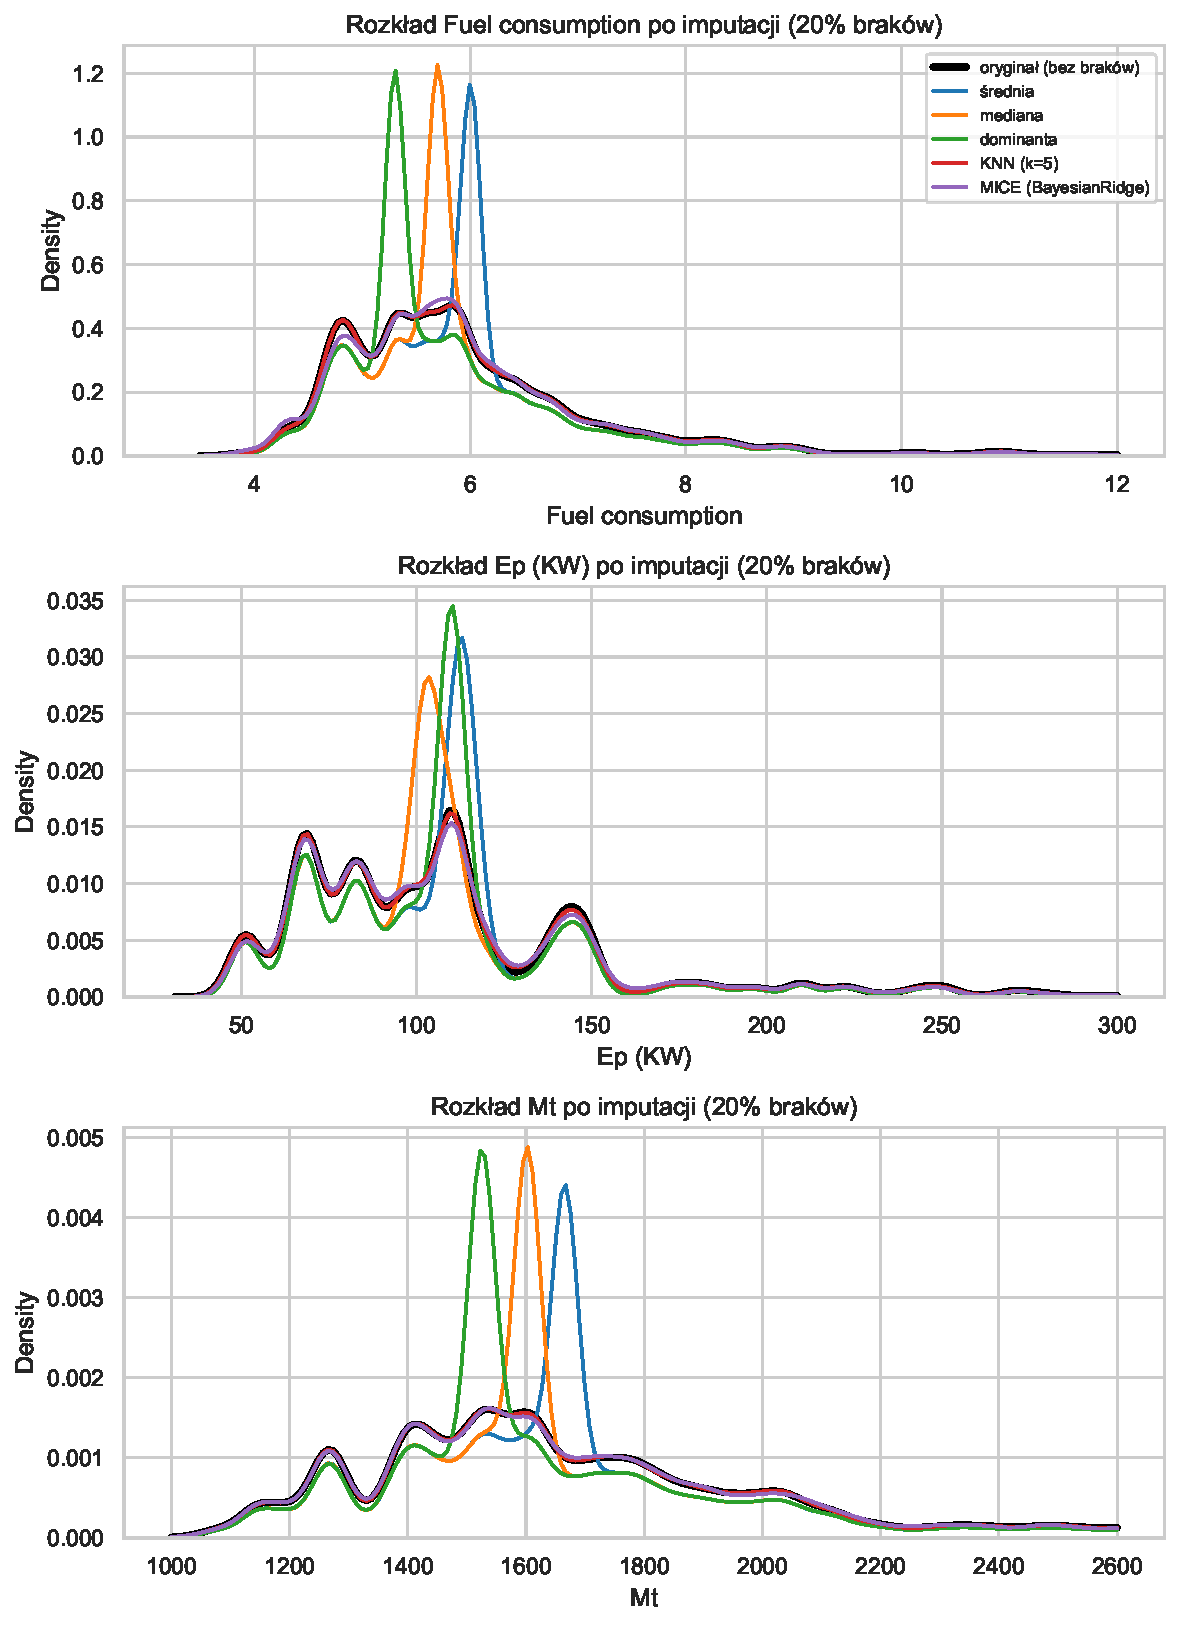
\includegraphics[width=\columnwidth]{imputation_distributions}
\caption{Rozkłady katalogowego zużycia paliwa, mocy i masy testowej po
imputacji 20\% sztucznych braków; czarna linia -- dane oryginalne.}
\label{fig:imp}
\end{figure}

\subsection{Transformacje i skalowanie}
Logarytm zmniejsza skośność cech liczbowych (rozdz.~2.2). Porównano
standaryzację i skalowanie min-max. Wybrano standaryzację, bo min-max ściska
większość obserwacji do wąskiego przedziału przez pojedyncze skrajne wartości,
których świadomie nie usuwaliśmy. Skalowanie jest konieczne dla KNN i MICE.
Modele drzewiaste i nieregularyzowana regresja liniowa są na nie niewrażliwe.

\subsection{Modele bazowe}
Porównano pięć modeli bazowych:
\begin{enumerate}[leftmargin=*,itemsep=1pt]
\item stała -- mediana zużycia paliwa ze zbioru treningowego,
\item katalogowe zużycie paliwa (przy braku -- przeliczone z emisji CO$_2$),
\item skorygowane katalogowe zużycie paliwa -- regresja
$y=a+b\cdot\text{katalogowe}$ osobno w 4 segmentach,
\item regresja liniowa na pełnym potoku,
\item \texttt{HistGradientBoostingRegressor} (gradientowe wzmacnianie drzew
decyzyjnych na histogramach cech) z parametrami domyślnymi -- podstawowy model
nieliniowy bez strojenia.
\end{enumerate}

Wyniki na walidacji przedstawia tab.~\ref{tab:baseline}. Samo katalogowe
zużycie paliwa jest gorsze nawet od stałej mediany, bo systematycznie zaniża
spalanie o 1,2\lkm. Prosta korekta usuwa większość tego błędu: współczynnik $b$
wynosi ok.\ 1,10 dla diesla i 1,19 dla benzyny, czyli luka rośnie
proporcjonalnie do zużycia paliwa. \texttt{HistGradientBoosting} poprawia
skorygowane katalogowe zużycie paliwa o 0,053\lkm{} (8\%) i niemal całkowicie
usuwa bias. Poprawa występuje we wszystkich segmentach, najmniejsza jest dla
diesli spalinowych.

Wszystkie egzemplarze tej samej wersji auta (ten sam model, silnik, masa,
kraj i rok) mają identyczne cechy, więc model może dla nich przewidzieć tylko
jedną wartość. Najlepszą możliwą jest typowe zużycie paliwa tej wersji. Aby
oszacować dolną granicę błędu, policzono MAE „wyroczni”: predykcji równej
medianie rzeczywistego zużycia paliwa w obrębie wersji, wyznaczonej na samej
walidacji (niemożliwe w praktyce, tylko do interpretacji). Wynosi ono
0,524\lkm. Jest to rozrzut między kierowcami identycznych aut, którego żadne
cechy techniczne nie wyjaśnią. Model zamyka więc ok.\ połowę odstępu między
skorygowanym katalogowym zużyciem paliwa a tą granicą.

\begin{table}[H]
\centering
\caption{Modele bazowe -- walidacja (trening na pełnym zbiorze treningowym).
MAE, RMSE i bias w l/100\,km; kat.\ -- katalogowe.}
\label{tab:baseline}
\footnotesize
\renewcommand{\arraystretch}{1.25}
\setlength{\tabcolsep}{4pt}
\begin{tabular}{@{}lrrrr@{}}
\toprule
Model & MAE & RMSE & $R^2$ & bias\\
\midrule
Stała (mediana) & 1,060 & 1,577 & 0,000 & $-0,002$\\
Katalogowe zużycie paliwa & 1,230 & 1,534 & 0,055 & $-1,206$\\
Skorygowane kat.\ zużycie paliwa & 0,639 & 0,943 & 0,643 & $-0,116$\\
Regresja liniowa & 0,618 & 0,918 & 0,661 & $-0,129$\\
HistGradientBoosting & \textbf{0,586} & \textbf{0,871} & \textbf{0,695} & $-0,032$\\
\bottomrule
\end{tabular}
\end{table}

\subsection{Stabilność i rozmiar zbioru treningowego}\label{sec:stab}
Dla 5 ziaren, które zmieniają przydział modeli aut do części, MAE modelu
\texttt{HistGradientBoosting} (uczonego na 1 mln wierszy) wynosi
$0,597 \pm 0,017$\lkm, a skorygowanego katalogowego zużycia paliwa
$0,645 \pm 0,018$\lkm. Model jest lepszy w każdym powtórzeniu, średnio
o 0,048\lkm.

Krzywa uczenia (rys.~\ref{fig:lc}) pokazuje, że przy bardzo małym zbiorze
(1\% treningu, 44 modele aut) najlepsza jest prosta korekta katalogowego
zużycia paliwa. Od ok.\ 5\% treningu wygrywa \texttt{HistGradientBoosting},
który poprawia się aż do pełnego zbioru (z 0,73 do 0,59\lkm) bez oznak
wypłaszczenia. Błąd na zbiorze treningowym jest zbliżony do walidacyjnego,
więc model nie jest przeuczony.

\begin{figure}[H]
\centering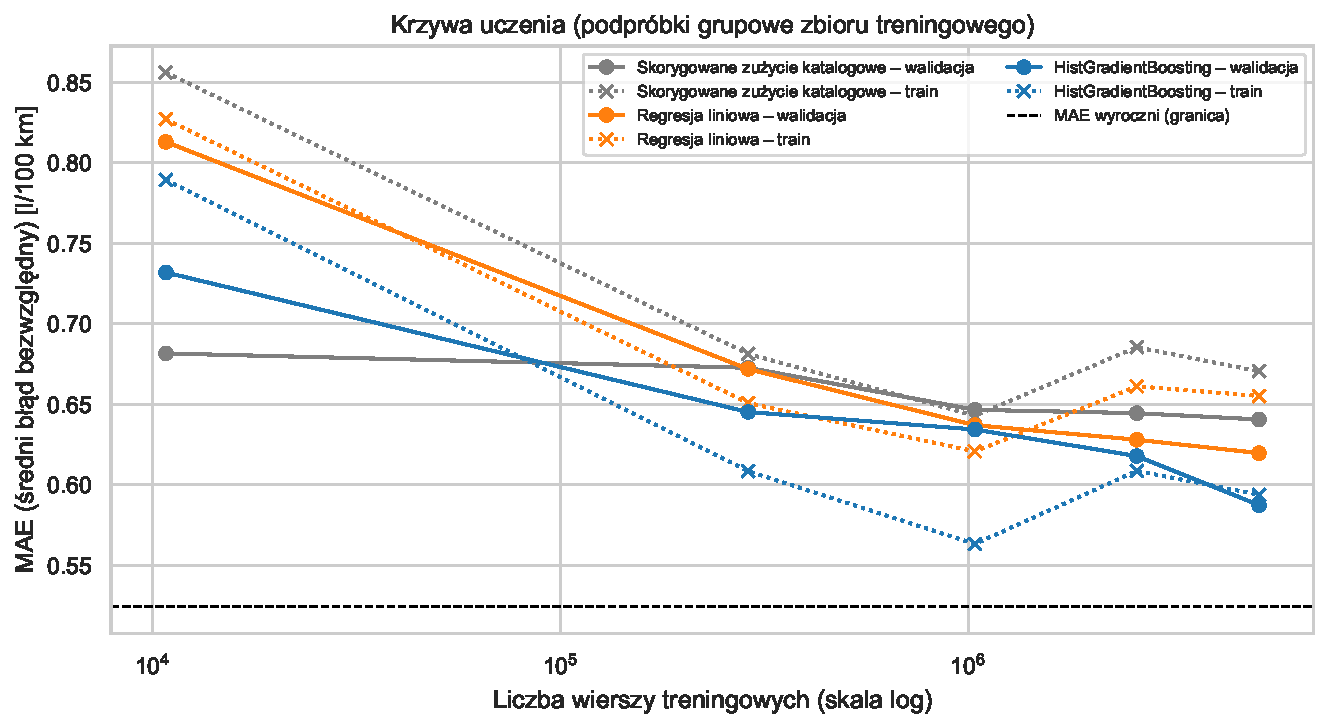
\includegraphics[width=\columnwidth]{learning_curve}
\caption{MAE w funkcji liczby wierszy treningowych (podpróbki grupowe:
1, 5, 20, 50 i 100\% zbioru treningowego); linia przerywana -- MAE wyroczni.}
\label{fig:lc}
\end{figure}

\subsection{Ocena na zbiorze testowym}
Zamrożoną procedurę oceniono jednorazowo na zbiorze testowym.
\texttt{HistGradientBoosting} osiąga MAE 0,614\lkm{} ($R^2$ 0,74), regresja
liniowa 0,659\lkm, skorygowane katalogowe zużycie paliwa 0,690\lkm, samo
katalogowe zużycie paliwa 1,161\lkm, a stała 1,190\lkm. Kolejność modeli jest
taka sama jak na walidacji. Wartości są nieco wyższe (inny zestaw modeli aut,
zgodnie z rozrzutem między ziarnami), a przewaga modelu nad skorygowanym
katalogowym zużyciem paliwa jest podobna (11\%).

\subsection{Wnioski}
Katalogowe zużycie paliwa bez korekty jest słabym predyktorem rzeczywistego
spalania, ale jego prosta korekta liniowa zmniejsza błąd niemal o połowę.
Podstawowy model nieliniowy bez strojenia poprawia ją o kolejne 8--11\%,
stabilnie dla różnych podziałów, a jego błąd (0,59--0,61\lkm) jest już bliski
granicy wynikającej z różnic między kierowcami (ok.\ 0,52\lkm).

\FloatBarrier
\bibliographystyle{plain}
\bibliography{bibliography}
\end{document}
